\subsection{Box-Cox regression model}

The Box-Cox transform, introduced by~\cite{box1964analysis}, is commonly used in statistics to correct the skewness and non-gaussianity of regression residuals. It is, therefore, a natural choice to improve the gaussianity of the residuals in the OGLASSO model and, consequently, improve the consistency in the significance of the interaction terms of the regression models used in the valuation of the VA portfolios.

The Box-Cox regression model is given by 

\begin{equation}
 Y(\lambda)=\beta_{0}+\beta_{1} X_{1}+\cdots+\beta_{k} X_{k}+\varepsilon,
\end{equation}
where $Y\left(\lambda \right)$ is the transformed response variable, $X_1 \ldots X_n$ the explanatory variables and $\varepsilon \sim N(0,\sigma^2)$. The transform, with parameters 
$\lambda=(\lambda_1, \lambda_2)$, is defined as 
\begin{equation}\label{boxcox}
 Y({\lambda})=\left\{\begin{array}{ll}{\frac{\left(Y+\lambda_{2}\right)^{\lambda_{1}-1}}{\lambda_{1}},} & {\text { if } \lambda_{1} \neq 0} \\ {\log \left(Y+\lambda_{2}\right),} & {\text { if } \lambda_{1}=0}\end{array}\right.
\end{equation}

As described in~\cite{box1964analysis}, the parameters $\lambda$ can be determined by maximizing the likelihood of the regression residuals. However, given the lack of appropriate software packages for the OGLASSO with the Box-Cox transform, we adopt a two-step procedure. First, we choose parameters to maximize the gaussianity of the FMVs, and then we fit the OGLASSO. Finally, we test the adequacy of the model by computing the FMVs for the entire portfolio of VA contracts, as in Section~\ref{sec:linear_model}.

The first parameter determined in our experiment is the shift $\lambda_2$, chosen to guarantee non-negative values for all transformed FMVs in the synthetic database. In the sequence,  values for $\lambda_1$ were chosen to maximize the gaussianity of the transformed FMVs in each representative portfolio. Using the estimated parameters, we found improvements in the symmetry of the transformed FMVs and also smaller deviations from the Gaussian distribution, as illustrated by the histograms and the QQ-plots in Figure~\ref{qqplot_transformed_fmv}. More importantly, after fitting the OGLASSO model for each representative portfolio, we obtain residuals that are significantly more Gaussian, as illustrated by the QQ-plots in Figure~\ref{qqplot_residuals_transformed_fmv} and their counterparts in Figure~\ref{residuals_oglasso}, where no transformations are used. 

Analysing the interaction matrices in figures~\ref{interactions} and~\ref{interactions_transformed_fmv}, we conclude that the detection of statistically significant interactions has also improved. First, we could observe an increase in the number of interactions for both representative portfolios. For the first, we notice an increased from 54 to 64 interactions, and from 46 to 76 for the second. The number of matching interactions (identified in both portfolios) has also increased, from 22 to 48. In addition, if we consider these matching interactions as correct, we also find an increase in accuracy: from 40\% to 75\% in the case of the first portfolio, and from 47\% to 63\% for the second.

The models estimated for both representative portfolios fit the transformed FMVs quite well, as their $R^2$ values are, respectively, 99.2\% and 98.6\%. In-sample predictions for the transformed FMVs and regular FMVs are illustrated in Figure~\ref{predictions_in_sample}, where they are compared against their correct values using QQ-plots. It is interesting to notice that, due to the Box-Cox transform, the transformed FMVs do not seem as concentrated as the non-transformed ones. 

We test the out-of-sample performance of the models by computing predictions for the entire data set of variable annuities. Results for both models can be found in Figure~\ref{predictions_out_of_sample}. Unfortunately, the improvements found in the in-sample results are not repeated in this test. Prediction errors are naturally larger in out-sample tests, however these seem to be inflated by the inverse Box-Cox transform, unexpectedly resulting in a poor out-of-sample performance. 

\begin{figure}[h!]
\makebox[\textwidth][c]{
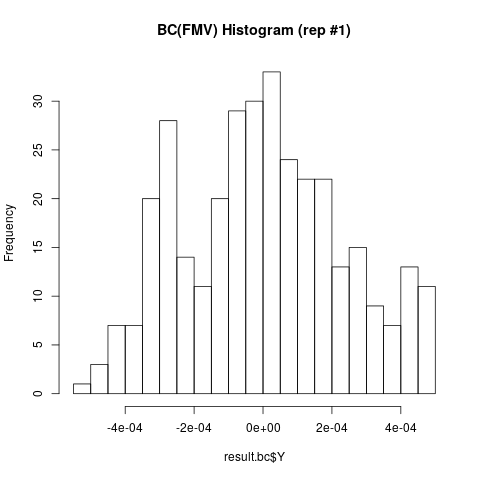
\includegraphics[scale=0.4]{pictures/boxcox_rep1_fmv_hist}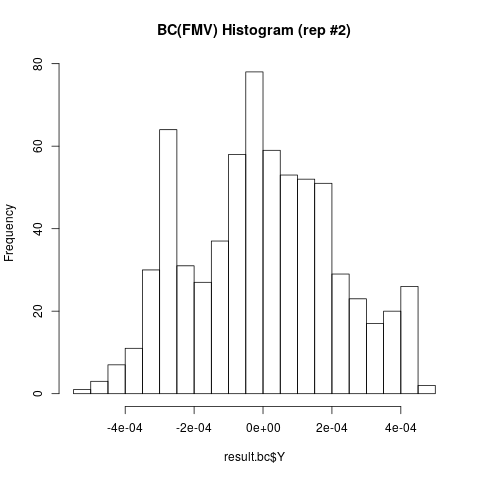
\includegraphics[scale=0.4]{pictures/boxcox_rep2_fmv_hist} 
}
\makebox[\textwidth][c]{
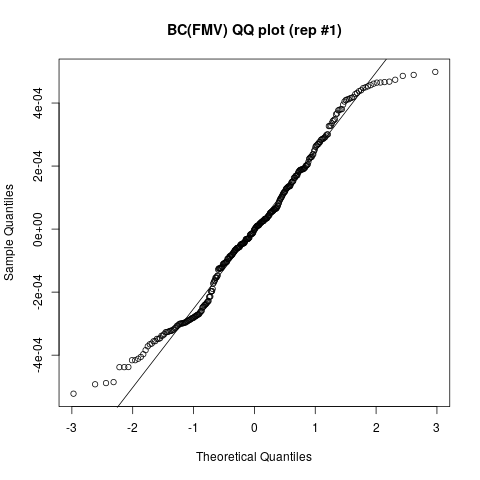
\includegraphics[scale=0.4]{pictures/boxcox_rep1_transformed_fmv_qqplot}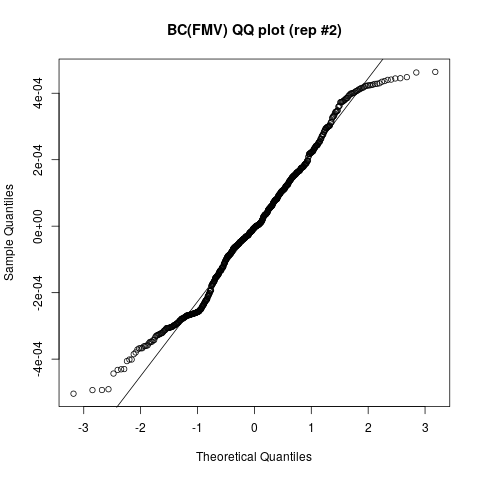
\includegraphics[scale=0.4]{pictures/boxcox_rep2_transformed_fmv_qqplot} 
}
\caption{Histograms and QQ-plots of transformed fair market values of contracts in the representative portfolios.}\label{qqplot_transformed_fmv}
\end{figure}


\begin{figure}[h!]
\makebox[\textwidth][c]{
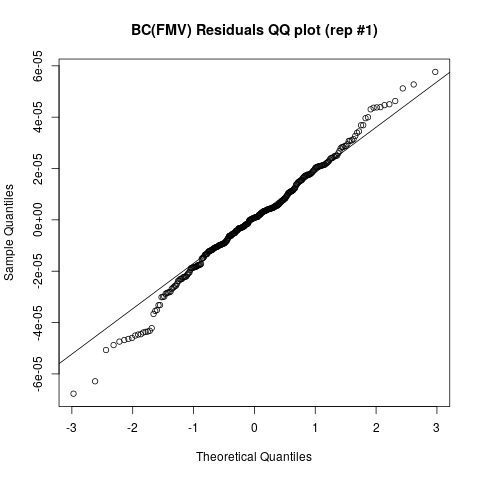
\includegraphics[scale=0.4]{pictures/boxcox_rep1_transformed_residuals_qqplot}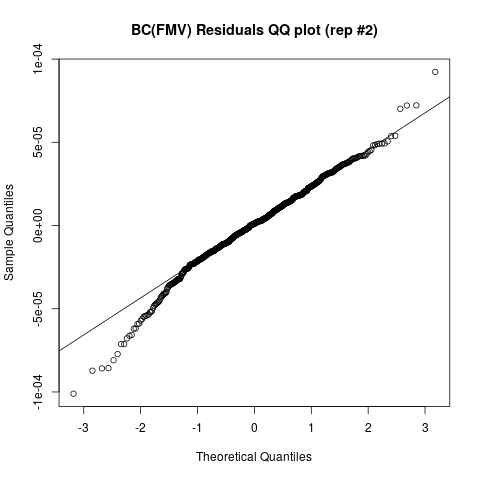
\includegraphics[scale=0.4]{pictures/boxcox_rep2_transformed_residuals_qqplot} 
}
\caption{QQ-plots of residuals for the models fitted on transformed fair market values.}\label{qqplot_residuals_transformed_fmv}
\end{figure}


\begin{figure}[h!]
\makebox[\textwidth][c]{
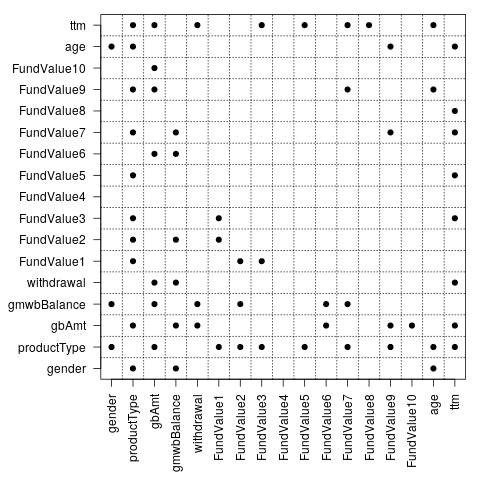
\includegraphics[scale=0.4]{pictures/boxcox_rep1_interactions}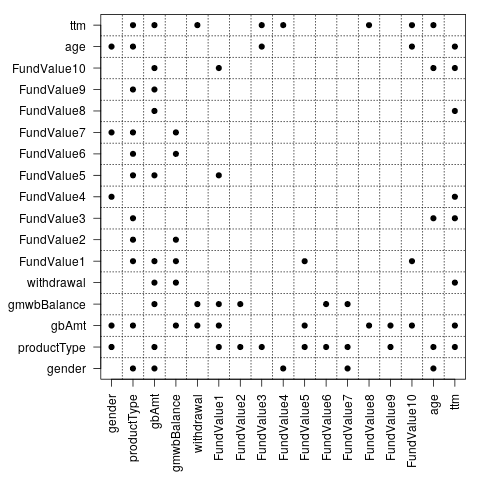
\includegraphics[scale=0.4]{pictures/boxcox_rep2_interactions} 
}
\caption{Interaction matrices for the models fitted on transformed fair market values.}\label{interactions_transformed_fmv}
\end{figure}

\begin{figure}[h!]
\makebox[\textwidth][c]{
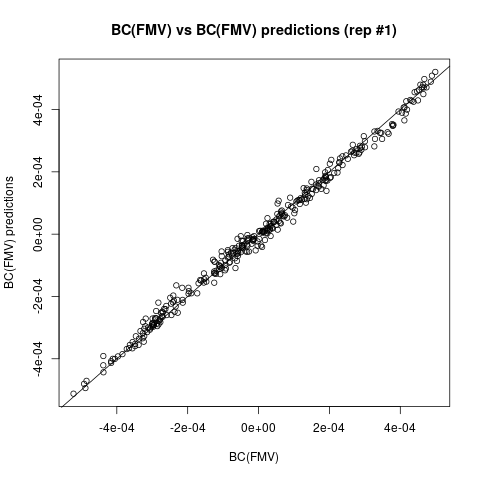
\includegraphics[scale=0.4]{pictures/boxcox_rep1_crossplot_transformed_fmv_predictions}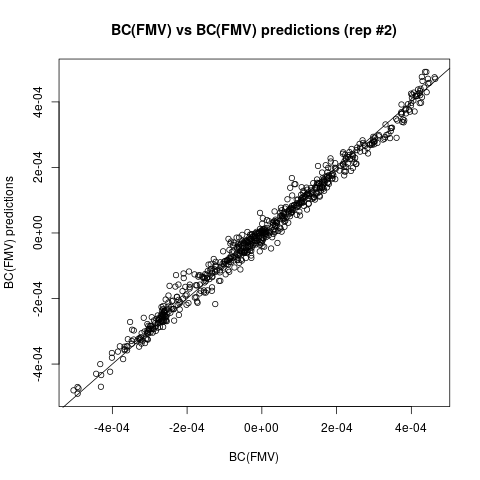
\includegraphics[scale=0.4]{pictures/boxcox_rep2_crossplot_transformed_fmv_predictions} 
}
\makebox[\textwidth][c]{
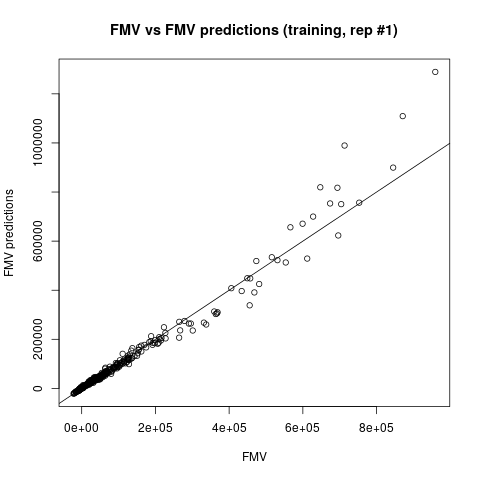
\includegraphics[scale=0.4]{pictures/boxcox_rep1_fmv_predict_train_median}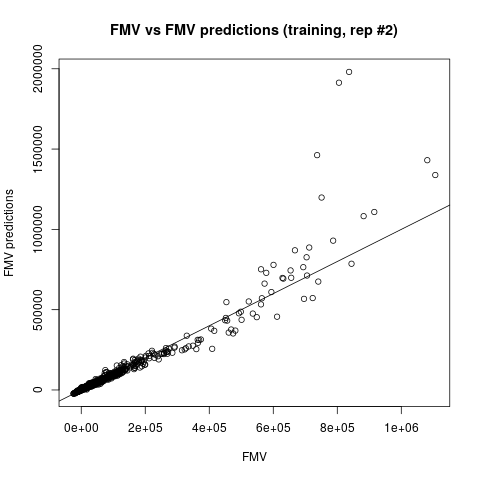
\includegraphics[scale=0.4]{pictures/boxcox_rep2_fmv_predict_train_median} 
}
%\caption{True FMV versus model predictions (training set) $r^2$: $0.9561$ and $0.8211$}\label{predictions_in_sample}
\caption{In-sample analysis of predictions for transformed fair market values (on top) and fair market values (below). The illustrated QQ-plots compare predicted values against the correct ones, available in the data set of variable annuity contracts.}\label{predictions_in_sample}
\end{figure}

\begin{figure}[h!]
\makebox[\textwidth][c]{
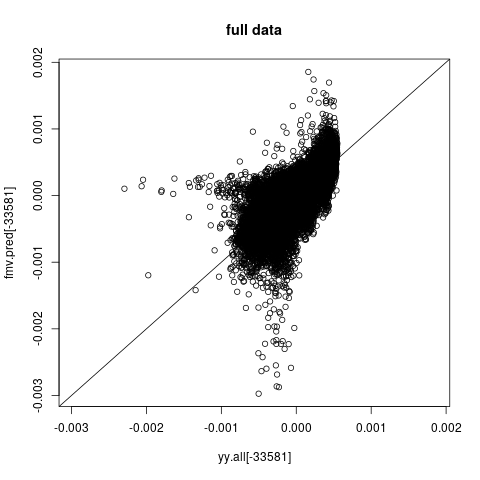
\includegraphics[scale=0.4]{pictures/boxcox_rep1_crossplot_transformed_fmv_predictions_all_data}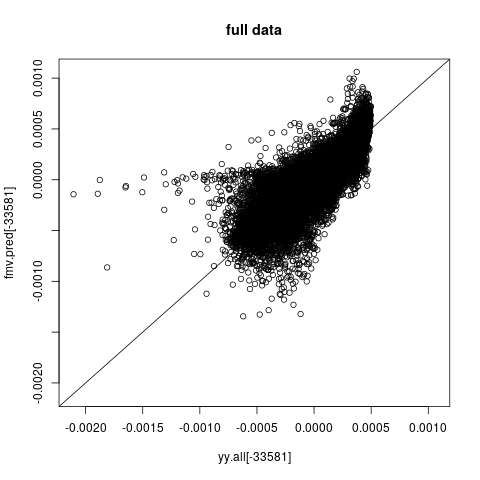
\includegraphics[scale=0.4]{pictures/boxcox_rep2_crossplot_transformed_fmv_predictions_all_data} }
%\caption{True transformed FMV versus model predictions (all data) $r^2$: $0.7788$ and $0.8616$}\label{predictions_transformed_out_of_sample}
%\end{figure}

%\begin{figure}[h!]
    \makebox[\textwidth][c]{
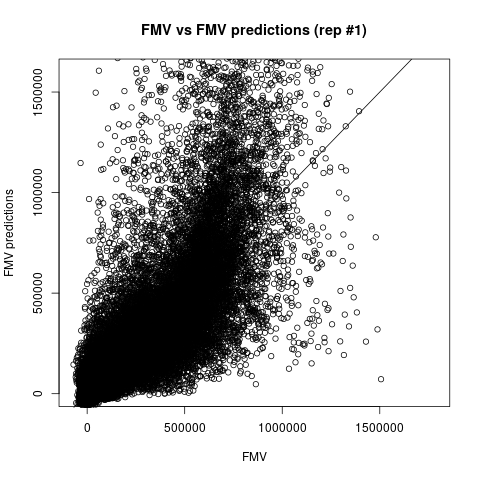
\includegraphics[scale=0.4]{pictures/boxcox_rep1_fmv_predictions_all_median}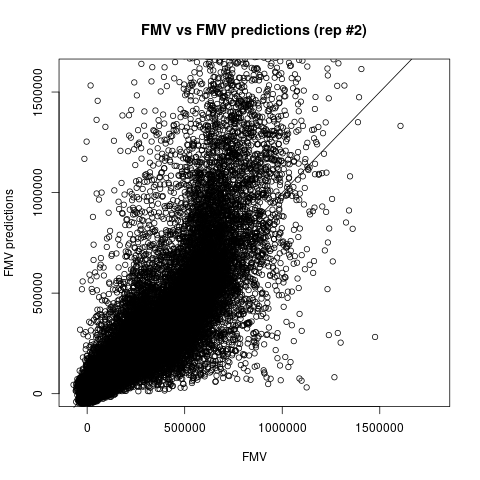
\includegraphics[scale=0.4]{pictures/boxcox_rep2_fmv_predictions_all_median} 
}
\caption{Out-of-sample analysis of predictions for transformed fair market values (on top) and fair market values (below). The illustrated QQ-plots compare predicted values against the correct ones, available in the data set of variable annuity contracts.}\label{predictions_out_of_sample}
\end{figure}

